\begin{tabular}{c c c}
	\adjustbox{valign=t}{			
		\begin{tikzpicture}
			\tikzset{every leaf node/.style={font=\sffamily}}
			\Tree
			[.{A} ]
		\end{tikzpicture}
	} % \adjustbox
	&
	\adjustbox{valign=t}{	
		\begin{tikzpicture}
			\tikzset{every leaf node/.style={font=\sffamily}}
			\Tree
			[.{B} 
				[.{C} ]
			]
		\end{tikzpicture}
	} % \adjustbox
	&
	\adjustbox{valign=t}{	
		\begin{tikzpicture}
			\tikzset{every leaf node/.style={font=\sffamily}}
			\Tree
			[.{0}
				[.$1$
					[.$3$  ]
					[.$4$  ]
					[.$5$  ]
				]
				[.$2$
					[.$6$ ]
					[.$7$ 
						[.$8$ ]
						[.$9$ ]
					]
				]
			]
		\end{tikzpicture}
	} % \adjustbox
\end{tabular}
